\chapter{The Backpropagation Algorithm}

\section{The Backpropagation Equations}

Before we describe anything, we briefly recap notation. We let
$C$ denote the cost function and $\sigma$ the activation function
of the neurons.
\begin{enumerate}
    \item $w_{j k}^{l}$ is the weight of the link between the $j$th
        neuron in layer~$l$ and the $k$th neuron in layer~$l - 1$.
    \item $b_j^l$ is the bias of neuron $j$ in layer~$l$.
    \item $z_{j}^l$ is the weighted input to neuron~$j$ in layer~$l$.
    \item $a_j^{l} = \sigma(z_{j}^l)$ is the activation of neuron~$j$ in
        layer~$l$.
    \item $\delta_{j}^{l} := \partial C / \partial z_{j}^{l}$ is
        the ``error'' of neuron~$j$ in layer~$l$.
\end{enumerate}

Using this notation, we may write the weighted output to neuron~$j$
in the $l$th layer as:
\[
    z_{j}^{l} = \sum_{k} w_{j k}^l a_{k}^{l - 1} + b_{j}^l =
                \sum_{k} w_{j k}^l \sigma (z_{k}^{l - 1}) + b_{j}^l,
\]
where the index~$k$ runs over all neurons in layer~$l - 1$ and
$2 \leq l \leq L$. Symbols such as $w^{l}$, $b^{l}$, $a^{l}$ without
subscripts refer to either matrices or vectors as the case may be.
For example, $w^{l}$ refers to the matrix whose $(j, k)$th element
is $w_{j k}^{l}$. This matrix has as many rows as there are neurons
in the $l$th layer and as many columns as there are neurons in
layer~$l - 1$. The symbol~$b^{l}$ refers to the vector of
biases~$b_{j}^l$ of the neurons in layer~$l$; similarly, $a^{l}$
refers to the vector of activations~$a_{j}^l$ of the neurons in
layer~$l$.

To understand why it makes sense to call
$\delta_{j}^{l} := \partial C / \partial z_{j}^{l}$  the ``error,'' consider a
small change $\Delta z_j^l$ in $z_j^l$. Then the change in the cost function $C$
as a result of this change in $z_j^l$ is $\partial C / \partial z_j^l \cdot \Delta z_j^l$.
If $\partial C / \partial z_{j}^{l} > 0$, then the cost increases as we increase
$\Delta z_j^l$; thus to reduce the cost, we must choose $\Delta z_j^l < 0$. Similarly,
if $\partial C / \partial z_{j}^{l} < 0$, then the cost increases if $\Delta z_j^l < 0$
and in order to reduce cost, we should select $\Delta z_j^l > 0$. Finally, if
$\partial C / \partial z_{j}^{l} \approx 0$, then changes in $z_j^l$ do not
affect the final cost. Thus $\partial C / \partial z_{j}^{l}$ indicates how we
should change the input $z_j^l$ to the $j$th neuron in layer~$l$.

We will derive the complete set of backpropagation equations in four steps. In what
follows, we will assume that the cost function $C$ is the usual quadratic cost.
\[
    C(x) = \frac{1}{2} \norm{y - a^L(x)}^2 = \frac{1}{2} \sum_{k} (y_k - a_k^L)^2.
\]
\subsubsection{Step I. Error of the Output Layer}
Let us consider the $j$th neuron in the last layer~$L$. The ``error'' $\delta_j^L$
of this neuron is given by
\begin{equation}
\label{eqn:individual_error}
    \delta_j^L := \frac{\partial C}{\partial z_j^L}
    = \frac{\partial C}{\partial a_j^L} \frac{\partial a_j^L}{\partial z_j^L}
    = \frac{\partial C}{\partial a_j^L} \frac{\partial \sigma(z_j^L)}{\partial z_j^L}
    = \frac{\partial C}{\partial a_j^L} \sigma'(z_j^L).
\end{equation}
Now $\partial C / \partial a_j^L = a_j^L - y_j$ and so
$\delta_j^L = (a_j^L - y_j) \sigma'(z_j^L)$. Assuming that there are $k$ neurons
in layer~$L$, we may write $\delta^L$, the vector of all the errors from layer~$L$,
as follows:
\begin{equation}
    \delta^L =
    \begin{pmatrix}
        \sigma'(z_1^L)  & 0              & \cdots & 0 \\
        \vdots          & \vdots         & \ddots & \vdots  \\
        0               & 0              & \cdots & \sigma'(z_k^L)
    \end{pmatrix}
    \begin{pmatrix}
        \frac{\partial C}{\partial a_1^L} \\
        \vdots \\
        \frac{\partial C}{\partial a_k^L}
    \end{pmatrix}
\end{equation}

\subsubsection{Step II. $\delta^l$ in terms of $\delta^{l + 1}$}
Now that we know what the error terms are in the final layer, we would
like to ``backpropagate'' these errors from the final layer to the first layer
of the network. In particular, we want to compute the errors in
layer~$l$ from the errors in layer~$l + 1$.

Let us assume that there are $p$ neurons in layer~$l$ and $q$ neurons in layer~$l + 1$.
What we would like to show is that:
\begin{equation}
\label{eqn:backprop_error}
\delta^l = \diag (\sigma'(z_1^l), \ldots, \sigma'(z_p^l)) \cdot \trans{(w^{l + 1})} \cdot \delta^{l + 1}.
\end{equation}
On the righthand side of the above equation, the diagonal matrix
$\diag (\sigma'(z_1^l), \ldots, \sigma'(z_p^l))$ has order~$p \times p$, the
matrix~$w^{l + 1}$ has order $q \times p$ and $\delta^{l + 1}$ has order $q \times 1$,
so that at least the order of $\delta^{l}$ correctly evaluates to $p \times 1$.
\begin{figure}[ht]
\begin{center}
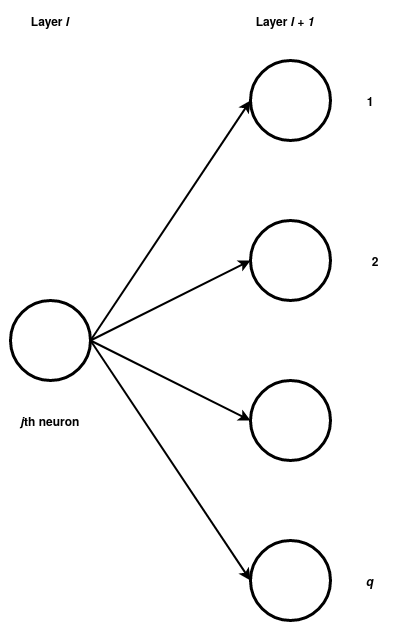
\includegraphics[scale=0.3]{twolayers.png}
\end{center}
\end{figure}

From~(\ref{eqn:individual_error}), we know that the error of the $j$th neuron in
layer~$l$ is given by
$\delta_j^l = \sigma' (z_j^l) \cdot \partial C / \partial a_j^l$. The output from
the $j$th neuron is fed to all neurons in layer~$l + 1$. Thus if we were to modify
the input weights to the $j$th neuron, its output would change and that would have a
cascading effect on the rest of the network. We wish to evaluate
how a change in the outputs of neuron~$j$ in layer~$l$ affects the output of
the neurons in layer~$l + 1$, assuming that all other weights in the network remain
fixed.
\begin{align}
\frac{\partial C}{\partial a_j^l}
    & = \sum_{k = 1}^q \frac{\partial C}{\partial z_k^{l + 1}} \cdot \frac{\partial z_k^{l + 1}}{\partial a_j^l} \nonumber \\
    & = \sum_{k = 1}^q \delta_k^{l + 1} \cdot  \frac{\partial z_k^{l + 1}}{\partial a_j^l}.
\end{align}
Now $z_k^{l + 1} = \sum_{i = 1}^p w_{k i}^{l + 1} \cdot a_i^l + b_k^{l + 1}$ and so
$\partial z_k^{l + 1} / \partial a_j^l = w_{k j}^{l + 1}$. Therefore,
\begin{equation}
    \frac{\partial C}{\partial a_j^l} = \sum_{k = 1}^q \delta_{k}^{l + 1} \cdot w_{k j}^{l + 1}.
\end{equation}
We can now write the error of the $j$th neuron in layer~$l$ as:
\begin{equation}
    \delta_j^l =  \sigma' (z_j^l) \cdot \sum_{k = 1}^q \delta_{k}^{l + 1} \cdot w_{k j}^{l + 1}.
\end{equation}
The above equation in matrix-form is precisely Equation~(\ref{eqn:backprop_error}).

\subsubsection{Step III. Evaluating $\partial C / \partial b_j^l$}
This is straightforward now.
\begin{equation}
    \frac{\partial C}{\partial b_j^l} =
    \frac{\partial C}{\partial z_j^l} \cdot \frac{\partial z_j^l}{\partial b_j^l} =
    \frac{\partial C}{\partial z_j^l} = \delta_j^l.
\end{equation}

\subsubsection{Step IV. Evaluating $\partial C / \partial w_{j k}^l$}
This is also a straightforward calculation.
\begin{equation}
    \frac{\partial C}{\partial w_{j k}^l} =
    \frac{\partial C}{\partial z_j^l} \cdot \frac{\partial z_j^l}{\partial w_{j k}^l} =
    \delta_j^l \cdot \frac{\partial}{\partial w_{j k}^l} \left (\sum_{i = 1}^p w_{j i}^l a_i^{l - 1} + b_j^l \right ) =
    \delta_j^l \cdot a_k^{l - 1}.
\end{equation}

We may write the backpropagation equations as:
\begin{equation}
\boxed{
\setlength{\jot}{12pt}
\begin{aligned}
    \delta^{L} & = \nabla_{a^L} C \odot \sigma'(z^L) \\
    \delta^{l} & = ( \trans{(w^{l + 1})} \delta^{l + 1} ) \odot \sigma'(z^l) \\
    \frac{\partial C}{\partial b_j^{l}} & = \delta_{j}^l := \frac{\partial C}{\partial z_j^l}\\
    \frac{\partial C}{\partial w_{j k}^l} & = a_{k}^{l - 1} \delta_{j}^l
\end{aligned}
}
\end{equation}
\section{Backpropagation Applied to Gradient Descent}

The backpropagation procedure calculates the gradient of the cost
function~$C$ with respect to a single input example. To make use of
backprop in the context of stochastic gradient descent, we need to take
the mean of the gradient computed over all examples in a mini batch.
Let's suppose that we have a mini batch with $m$ examples
$x_1, \ldots, x_m$.
\begin{enumerate}
    \item For each training example~$x$, set the input activation
        $a^1 (x)$ and perform the following steps:
        \begin{enumerate}
            \item \textbf{Feedforward.} For $2 \leq l \leq L$, set
                $z^l (x) = w^l a^{l - 1} (x) + b^l$ and
                $a^l (x) = \sigma (z^l (x))$.
            \item \textbf{Output Error.} Calculate
                $\delta^L (x) = \nabla_{a^L} C(x) \odot \sigma' (z^L (x) )$.
            \item \textbf{Backprop.} For $L - 1 \leq l \leq 2$,
                $\delta^l (x) = ( \trans{(w^{l + 1})} \delta^{l + 1} (x) )
                                    \odot \sigma' (z^l (x))$.
            \item \textbf{Gradients.} Calculate
            $ \frac{\partial C}{\partial b_j^{l}} (x) = \delta_{j}^l (x)$
            and $\frac{\partial C}{\partial w_{j k}^l} (x)
                    = a_{k}^{l - 1} \delta_{j}^l (x)$.
        \end{enumerate}
    \item \textbf{Gradient Descent.} For $L \leq l \leq 2$, set
        $w^l = w^l - \frac{\eta}{m} \sum_{x} \delta^{l} (x) \trans{(a^{l - 1} (x))}$
        and
        $b^l = b^l - \frac{\eta}{m} \sum_{x} \delta^l (x)$.
\end{enumerate}
